\chapter{Software Defined Networking}

SDN is often referred to as a ``radical new idea of networking''. It has been made to overcome many requirements and current network technology limitations which arose in the last years:
\begin{enumerate}
   \item[] \ul{The demand is increasing}
   \item Cloud computing
   \item Big Data
   \item Mobile traffic
   \item IoT
   \item[] \ul{\textit{Supply} also increasing}
   \item Network technologies capable of absorbing high load
   \item Performance of network devices increased
   \begin{enumerate}
      \item CPU speed
      \item Buffer capacity and speed
      \item etc...
   \end{enumerate}
   \item[] \ul{\textit{Traffic patterns}\footnote{Traffic patterns measure how traffic varies in time and space} have changed and became more dynamic and complex} 
   \note{This is the most critical aspect}
\end{enumerate}

\section{Motivations and Traffic Patterns}
Modern distributed applications typically access multiple databases and servers that
must communicate with each other, creating a lot of
\textit{``horizontal''} traffic between servers ---in addition to the \textit{``vertical''} client/server one--- which was initially neglectable, but now it is not.

Unified communications (UC) services are increasingly used within enterprises. Many communication services such as instant messaging (chat), presence
information, voice, mobility, audio, web and video traffic, must be \textit{integrated} into a unique service
delivery platform

Increasing use of cloud shifted traffic relegated in enterprise networks to remote clouds, causing unpredictable loads on enterprise routers.

Server virtualization, now a common practice, besides increasing the number of virtual machines (VMs) on a single physical server and corresponding communications, brings east-west traffic due to migration and remote storage access.

Summing up, up to $70\%$ of traffic in datacenters is now East West, and traditional three-tier \textit{access-aggregation-core} network architecture no longer fits the bandwidth traffic requirements.


\section{Layering}
Layering, as it is applied in TCP/IP stack, implies decomposing delivery into fundamental components, allowing independent but compatible innovation at each layer; it revealed itself to be pretty successful, however, \ul{many issues reside in the \textit{Network Control/Management Plane}}.

If in computer science usually many clean and elegant abstractions are used, network control instead is strongly related to hardware and verbose protocols, there are \textit{no} principles or abstractions guiding the process, making in general difficult managing traffic flows.

SDN helps providing some abstraction through a centralized view of the network.

\subsection{Network Layer}
\begin{itemize}
   \item \textbf{Forwarding} move packets from router’s input to appropriate router output
   \note{Data Plane}
   \item \textbf{Routing} determine route taken by packets from
   source to destination
   \note{Control Plane\\
   Traditionally it was implemented \textit{per-router}, with SDN instead is \textit{logically centralized}}
\end{itemize}

These are the two key tasks. In Fig. \ref{fig:sdn_planes} a comparison between the tradional and the SDN approaches.
\begin{figure}[htbp]
   \centering
   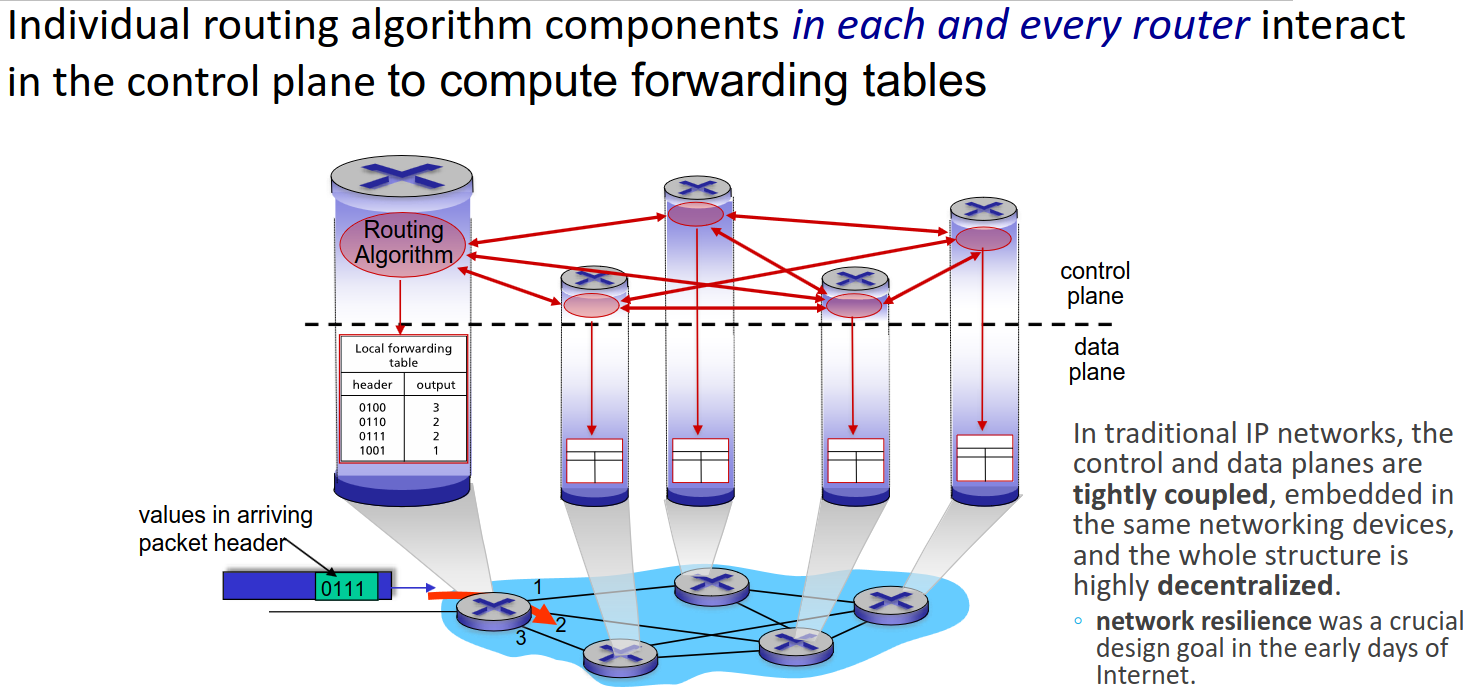
\includegraphics[width=0.45\columnwidth]{images/sdn_planes1.png}
   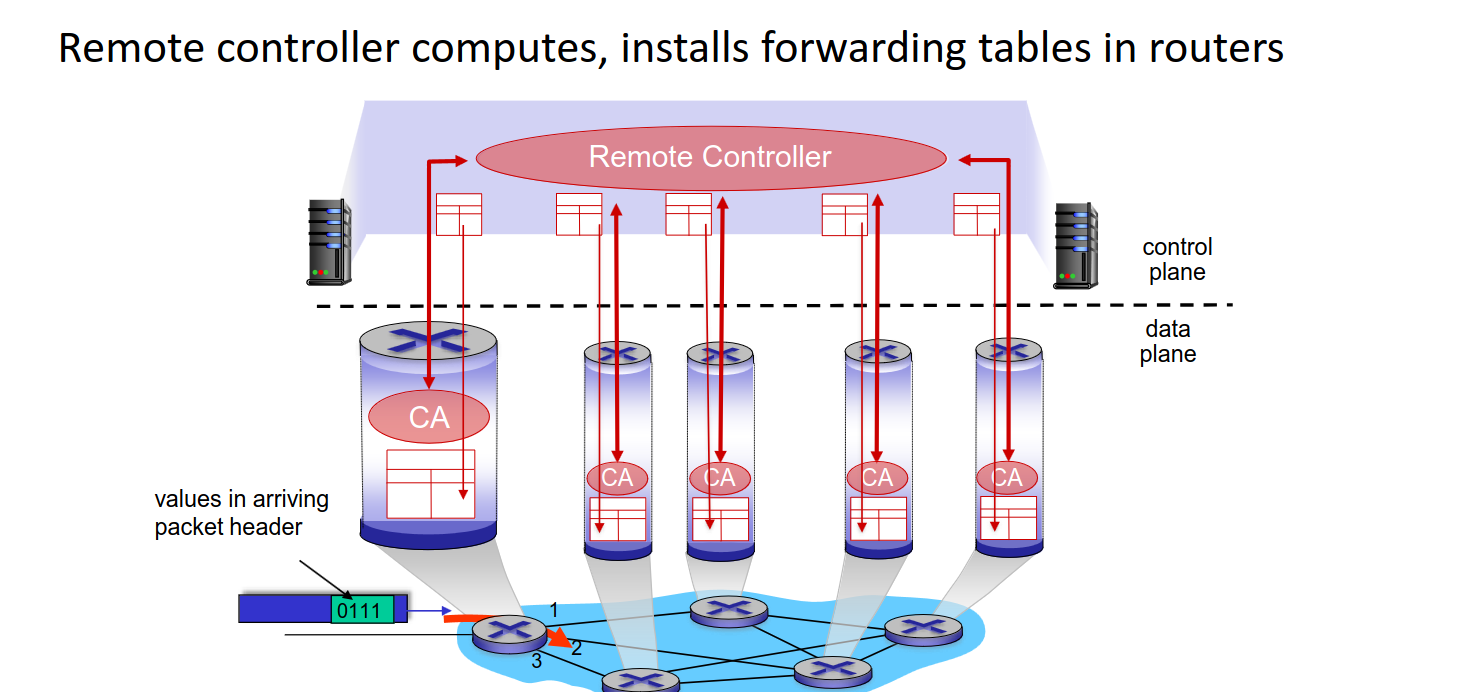
\includegraphics[width=0.45\columnwidth]{images/sdn_planes2.png}
   \caption{Traditional vs SDN}
   \label{fig:sdn_planes}
   \end{figure}
In Internet early days, \textbf{resiliency} was a key issue, so the network was designed to be decentralized and distributed, with data and control tightly coupled and embedded in the same ---routers--- networking devices.\\
However, this design does not allow to arbitrarily choose the traffic paths with ease: the only way to do so is to change the link weights, and waiting for a recomputation of the routing tables, which is somewhat far from being considered ``control''.

\section{SDN Architecture}
\begin{paracol}{2}
   \textbf{Data-plane switches} are fast, simple, commodity switches implementing generalized data-plane forwarding in hardware, and generally provide API for table-based switch control, e.g. \texttt{OpenFlow}.

   \textbf{SDN controller} (network OS) maintain network state information and interacts with network control applications ``above'' via northbound API, and with switches using ``below'' via southbound API.
   They are implemented as distributed system for performance, scalability, fault-tolerance, robustness.

   \textbf{Network-control apps} are ``brains'' of control, they implement control functions using lower-level services. They are \textit{unbundled}, meaning that they may be provided by a $3^{rd}$ party different from routing vendor or SDN controller
   \switchcolumn
   \begin{figure}[htbp]
      \centering
      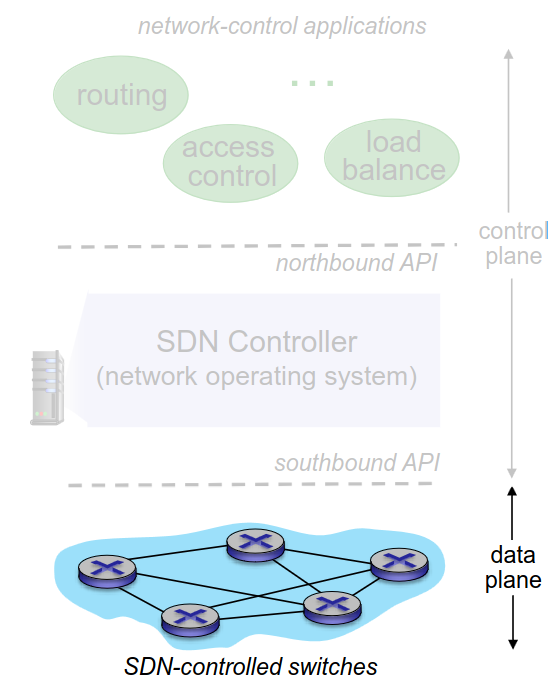
\includegraphics{images/sdn_planes3.png}
      \caption{SDN Layer Architectures}
      \label{fig:sdn_planes3}
   \end{figure}
\end{paracol}

\newpage
\subsection{Data Plane}
Resource or infrastructure layer providing a \textit{Forwarding Abstraction} made up of \textbf{forwarding devices} ---without embedded software to make autonomous decisions--- which perform the transport and processing of data according to decisions made by the SDN control plane.

\begin{paracol}{2}
   
   \colfill
   Inside the routers there is an \textbf{OpenFlow} \textbf{flow\footnotemark[1] table}.
   The pattern implemented is called \ul{\textit{``match+action''}} and is used to define the rules for packet processing. FOr each packet bits are analysed and compared to the rules in the flow table, when a match is found, the corresponding action is taken.
   \colfill
   \switchcolumn
   \begin{figure}[htbp]
   \centering
   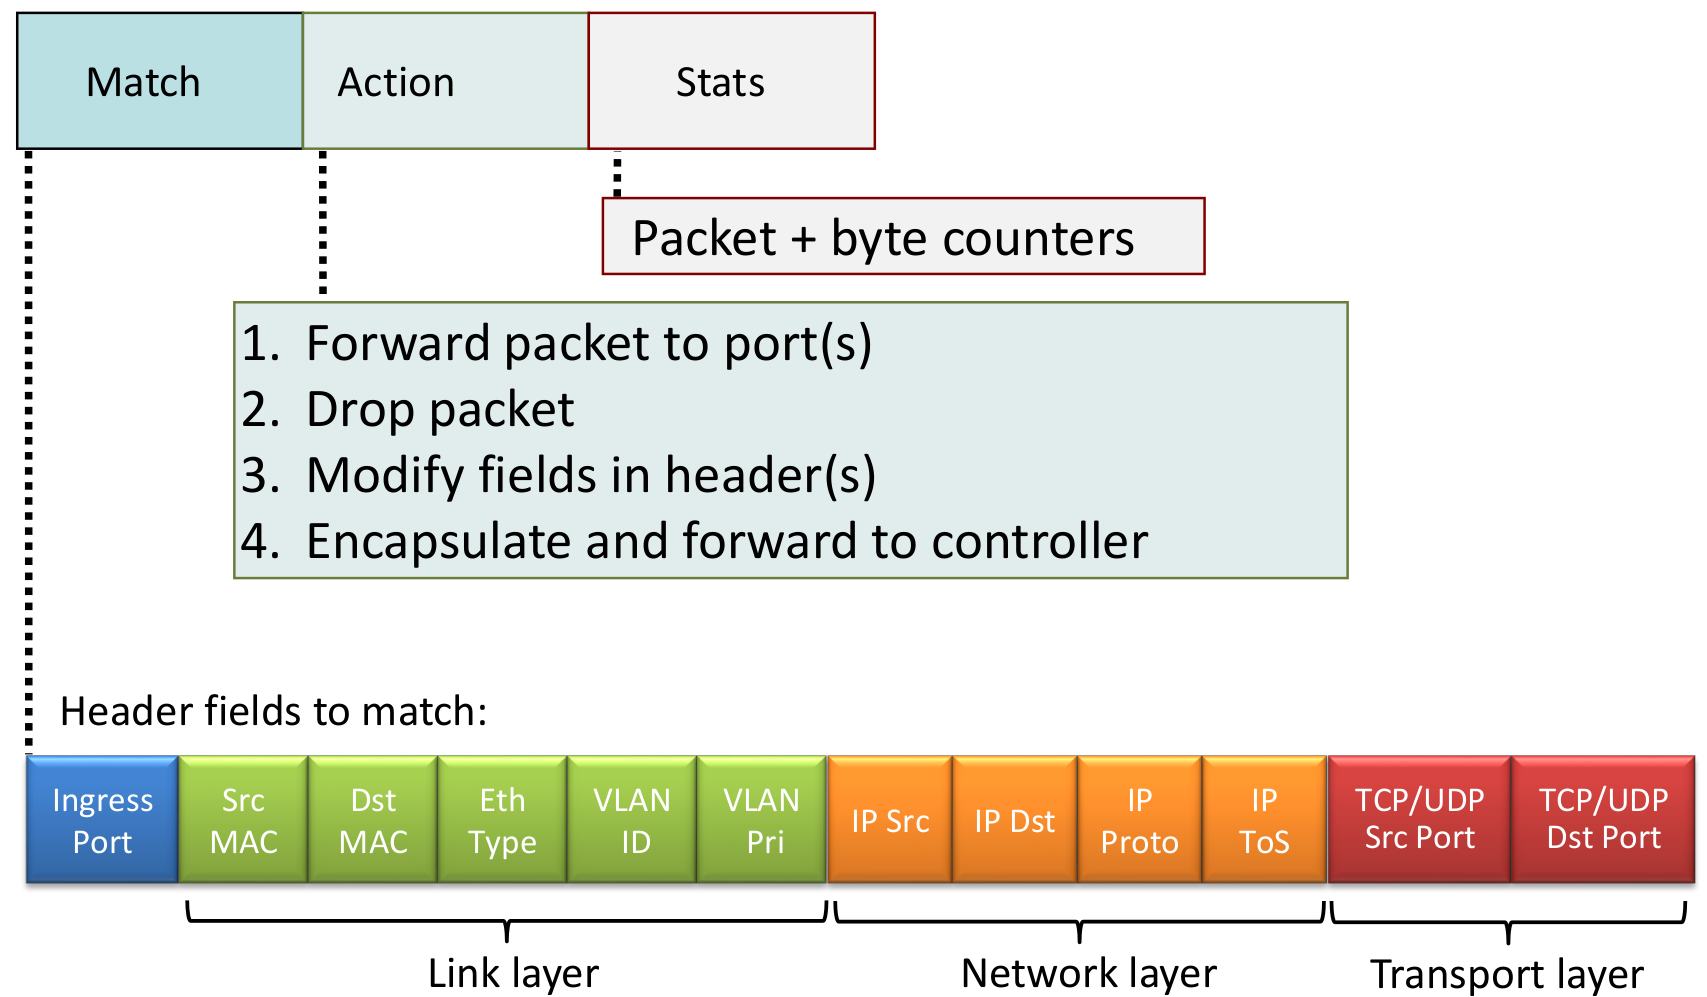
\includegraphics{images/openflow_table.png}
   \caption{OpenFlow table}
   \label{fig:openflow_table}
   \end{figure}
\end{paracol}

\begin{paracol}{2}
   \colfill
   Some simple forwarding rules are defined:
   \begin{itemize}
      \item \textit{Match}:
      Pattern values to be matched in packet header fields
      \item \textit{Actions}:
      Actions to be performed for matched packet: \texttt{drop, forward, modify} 
      \item \textit{Priority}:
      Used to disambiguate overlapping matching patterns
      \item \textit{Counters}:
      Typically used for \texttt{\#bytes} and \texttt{\#packets}   
   \end{itemize}
   \colfill

   \switchcolumn
   \begin{figure}[htbp]
      \centering
      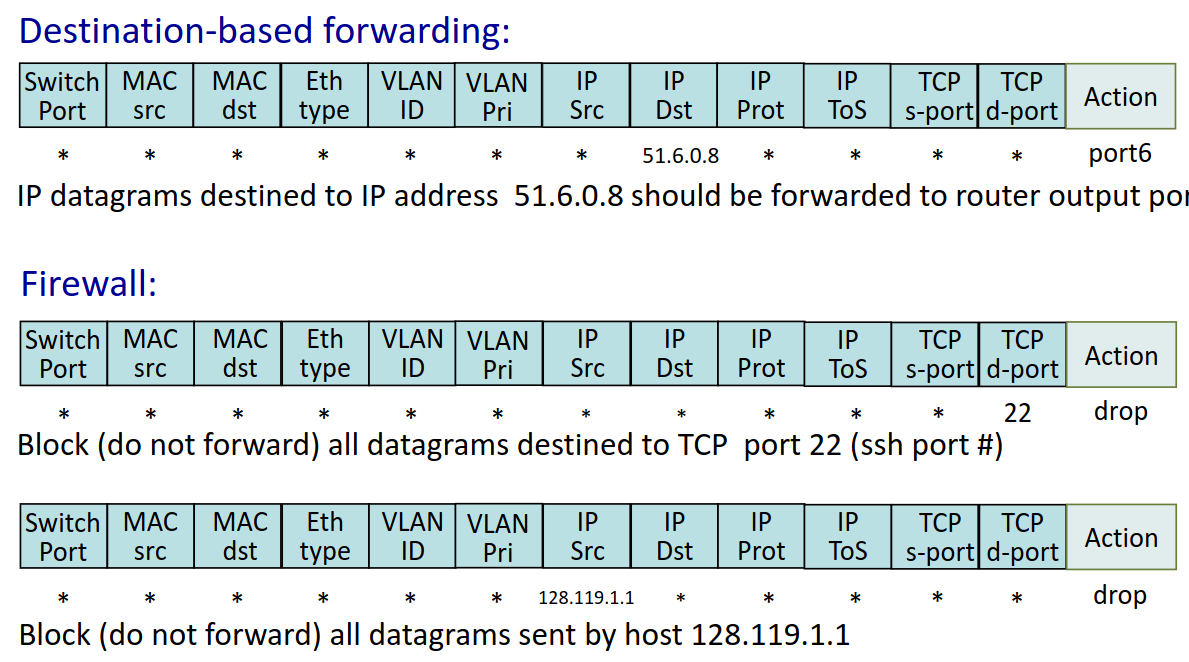
\includegraphics{images/openflow_rulesexamples.png}\\
      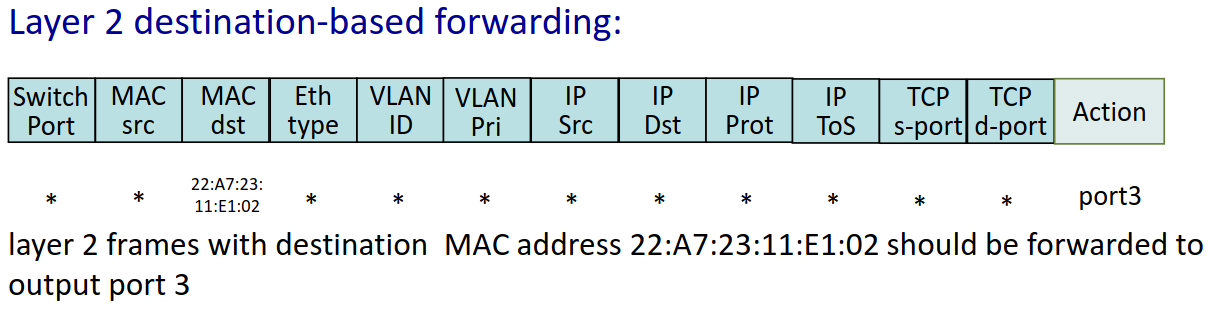
\includegraphics{images/openflow_rulesexamples1.png}
      \caption{OpenFlow rules examples}
      \label{fig:openflow_rulesexamples}
   \end{figure}to enable the
\end{paracol}

\footnotetext[1]{Defined by \textit{link}, \textit{network} and \textit{transport} layer fields}

\begin{figure}[htbp]
   \centering
   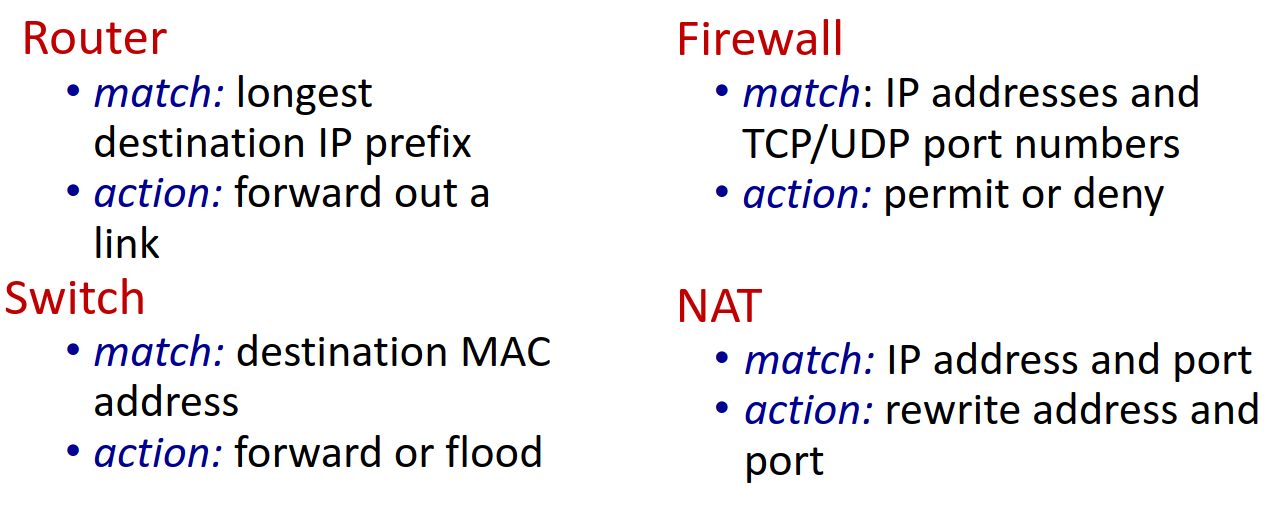
\includegraphics{images/openflow_matchaction.png}
   \label{fig:openflow_matchaction}
\end{figure}
The abstraction of \texttt{match+action} unifies different kinds of devices

\subsection{OpenFlow to control the Network Device}
Data Plane Network devices support, alongside the abovementioned rule-based formwarding capabilities, interaction with the SDN controller for management of forwarding rules, through OpenFlow switch protocol.

\begin{figure}[htbp]
   \centering
   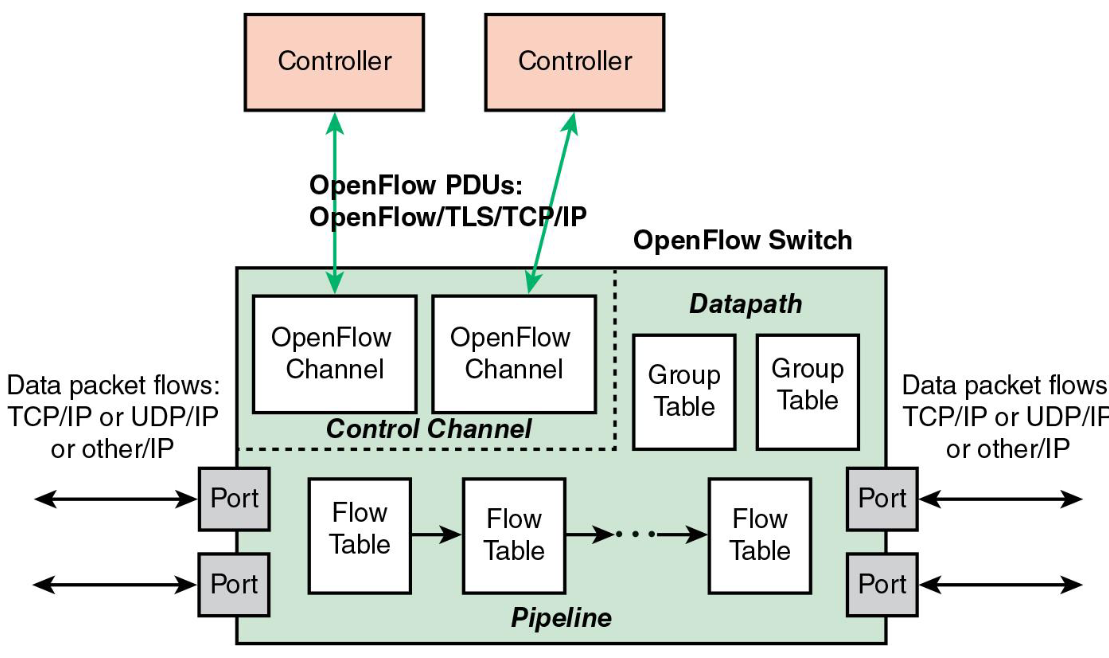
\includegraphics{images/openflow_switch.png}
   \caption{OpenFlow switch}
   \label{fig:openflow_switch}
\end{figure}
Through OpenFlow, the controller can add, update, and delete flowentries in tables, both reactively (in response to packets) and proactively.

A switch is made up of one or multiple pipelined flow tables, possibly allowing for considerable flexibility.
Instructions performed on a packet may explicitly direct it to another flow table (\texttt{Goto} instruction) and so on, until it is formwarded to an output port.
A packet may also be redirected to controller, enabling it to define a new flow for that and similar packets, or decide to drop the packet
\begin{figure}[htbp]
   \centering
   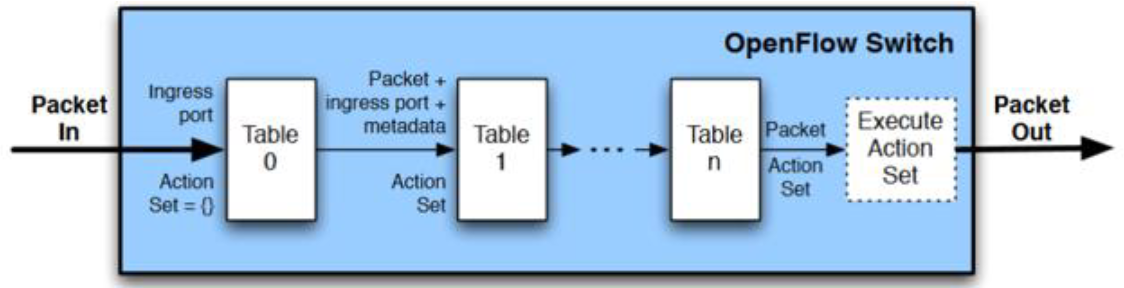
\includegraphics{images/openflow_switchtables.png}
   \caption{Multiple tables inside switch}
   \label{fig:openflow_switchtables}
\end{figure}


\section{Control Plane}
\begin{figure}[htbp]
   \centering
   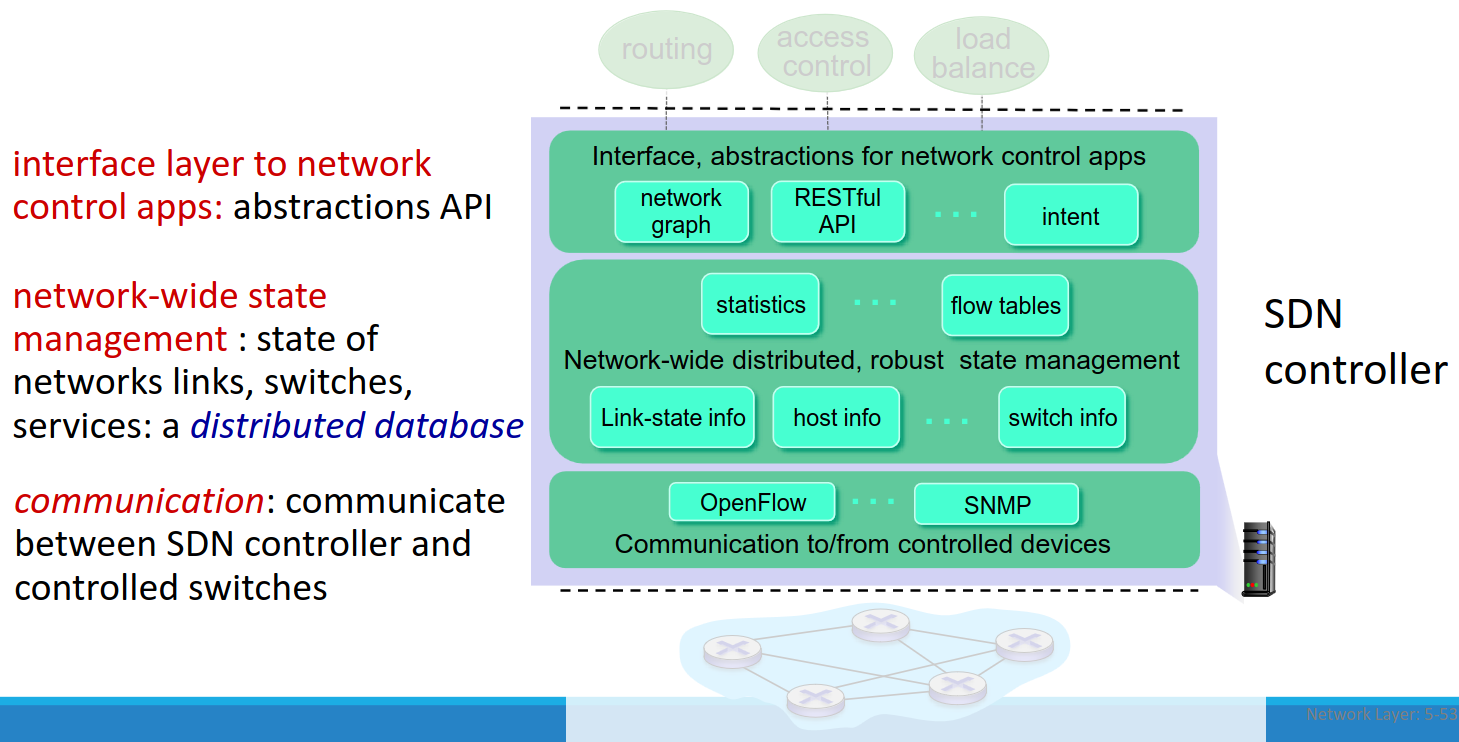
\includegraphics{images/openflow_controllerinside.png}
   \caption{Inside an OpenFlow controller}
   \label{fig:openflow_controllerinside}
\end{figure}
The Openflow protocol operates between acontroller and switches using TCP (optional encryption). There are three classes of OpenFlow messages:
\begin{enumerate}
   \item Controller-to-switch
   \begin{enumerate}
      \item \textit{Features}:
      controller queries switch features, switch replies
      \item \textit{Configure}:
      controller queries/sets switch configuration parameters
      \item \textit{Modify-state (FlowMod)}:
      add, delete, modify flow entries in the OpenFlow
      tables
      \item \textit{Packet-out}:
      controller can send this packet out of specific switch port
   \end{enumerate}
   \item Asynchronous (switch to controller) 
   \begin{enumerate}
      \item \textit{Packet-in}:
      transfer packet (and its control) to controller. See packet-out message from controller
      \item \textit{Flow-removed}:
      flow table entry deleted at switch
      \item \textit{Port status}:
      inform controller of a change on a port.
   \end{enumerate}
   \item Symmetric (misc.)
\end{enumerate} 
\note{Fortunately, network operators don't ``program'' switches by creating/sending OpenFlow messages directly; they use instead use higher-level abstraction at controller.}

\subsection{Link Failure scenario}
\begin{paracol}{2}
   
   \begin{figure}[htbp]
      \centering
      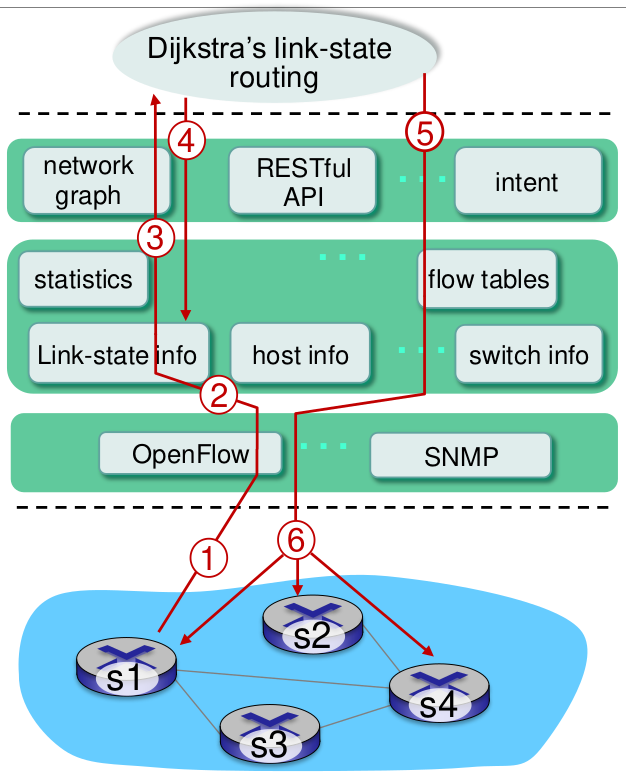
\includegraphics{images/sdn_linkdown.png}
      \caption{S1 loses the link (not displayed) with S2}
      \label{fig:sdn_linkdown}
      \end{figure}
   \switchcolumn
   \begin{enumerate}
      \item S1 detects link failure and uses OpenFlow port status message to notify controller.
      \item SDN controller receives OpenFlow message, and updates link status info.
      \item Dijkstra's routing algorithm gets called in this case
      \item The algorithm accesses enetwork graph info, link state info in controller, and computes new routes.
      \item Link state routing app interacts with flow-table-computation component in SDN controller, which computes the new flow tables for switches.
      \item The controller sends OpenFlow messages to install new tables in switches that need updating.
   \end{enumerate}   
   \end{paracol}


\section{Topology discovery and forwarding in the SDNs}
\subsection{Routing}
While traditionally the routing function is \textit{distributed} among the routers in a network, in an SDN controlled network, it makes sense to \ul{\textbf{centralize} the routing function within the SDN controller}, allowing it develop a consistent view of the network state for calculating shortest paths and implementing application-aware routing policies.\\
Thus, data plane switches are relieved of the processing and storage burden associated with routing, leading to improved performance.

The centralized routing application performes two tasks
\begin{itemize}
   \item \textbf{Link/Topology discovery}
   \begin{itemize}
      \item The routing function needs to be aware of links between data plane switches
      \item The topology discovery in OpenFlow domains currently is not standardized
   \end{itemize}
   \item \textbf{Topology manager}
   \begin{itemize}
      \item Maintains the topology information for the network
      \item calculates routes in the network (the shortest path between two data plane
      nodes or between a data plane node and a host)
   \end{itemize}
\end{itemize}

\subsection{Topology Discovery}
Every OF switch has initially set the IP address and TCP port of a controller to establish a connection as soon as the device is turned on; it also has preinstalled flow rules to route directly to the controller via a Packet-In message any message of the \textbf{Link Layer Discovery Protocol (LLDP)}, which is a neighbor discovery protocol of a single jump, i.e. it advertises its identity and capabilities and receives the same information from the adjacent switches.
\note{
   LLDP is vendor neutral and works at layer 2, using \textit{Ethernet} as ``transport'' protocol.
}

Switches send the LLDP messages (\textit{``frames''}) ---periodically at a given interval of time--- to discover the underlying topology by request of the controller.

\subsubsection{LLDP message content}
\begin{itemize}
   \item \texttt{Chassis ID}: identifier of switch sending the packet
   \item \texttt{Port ID}: identifier of the port through which the LLDP packet is sent
   \item \texttt{TTL}: time in seconds during which the information received in the LLDP
   packet is going to be valid.
   \item End of \texttt{LLDPDU}: indicates the end of the payload in the LLDP frame
\end{itemize}

\subsubsection{Discovery process}
\begin{enumerate}
   \item The controller generates a Packet-Out message per active port on each switch discovered on the network and encapsulates a LLDP packet inside each generated message.
   \item When an OF switch receives a LLDP message sent by the controller, it forwards the message by the appropriate Port ID included in the message to adjacent switches
   \item Upon receiving the messages by a port that is not the controller port, the adjacent switches encapsulate the packet within a Packet-In message addressed to the controller. Metadata is included in the message such as Switch ID, Port ID where the LLDP packet is received, among others
   \item When the packet comes back to the controller from an adjacent switch, the controller extracts this information, and then it knows a link exists between those switches
   \note{Switch ID and Port ID in the LLDP message and Switch ID and Port ID in metadata}
\end{enumerate}
\ul{This process is repeated for each switch.}

\section{Google B4 WAN}
There are two \textbf{backend backbones}, \texttt{B2} carrying internet facing traffic, and \texttt{B4} moving inter-datacenter traffic; the latter has grown a lot in the recent years.

B4 was needed for various reasons:
\begin{itemize}
   \item Not on the public Internet
   \item Cost effective network for high volume traffic
   \item Bursty/bulk traffic\footnote{\textit{``Burst''}: a group of packets with shorter interpacket gaps than packets arriving before or after that burst}
\end{itemize}

Flow types traversing backend backbones are:
\begin{itemize}
   \item User data copies
   \item Remote storage access
   \item Large-Scale data push synchronizing state across multiple data centers
\end{itemize}